\chapter[Event Simulation and Object Reconstruction]{Event Simulation and \protect\\Object Reconstruction}
\label{ch:evSimObjReco}
\epigraph{\emph{Nature isn't classical, dammit, and if you want to make a simulation of nature, you'd better make it quantum mechanical, and by golly it's a wonderful problem, because it doesn't look so easy.}} {Richard P. Feynman}

	The \ac{ATLAS} software framework Athena~\cite{TDR2005}, which is based on the Gaudi~\cite{Gaudi2000} framework developed by \ac{LHCb}~\cite{LHCb2008}, is used to reconstruct physics objects to be used by analysers, as the data collected and recorded by the \ac{ATLAS} detector requires processing. The Athena framework is capable of dealing with various aspects of the experiment software, \eg\ triggering or the processing of simulated data. Custom software, in particular \ac{MC} simulations, is used to simulate physics events used to model background and signal processes. These are produced through different stages, as shown in Figure~\ref{fig:workflow}, the last of which produces an analyser-friendly output. 

	In this chapter the stages will be briefly explained as it follows: event generation (Section~\ref{sec:evGen}); reconstruction of physics objects\footnote{A set of criteria needs to be applied in order to reconstruct the detected object as an ``electron'', ``photon'', ``muon'', ``jet'', etc.}, in both collected data and simulated \ac{MC} events (Section~\ref{sec:objReco}).%  Finally, a set of selection criteria are applied to reconstructed objects to identify those suitable for use in analysis, as detailed in Section~\ref{sec:objSel}.

	\begin{figure}
		\centering
		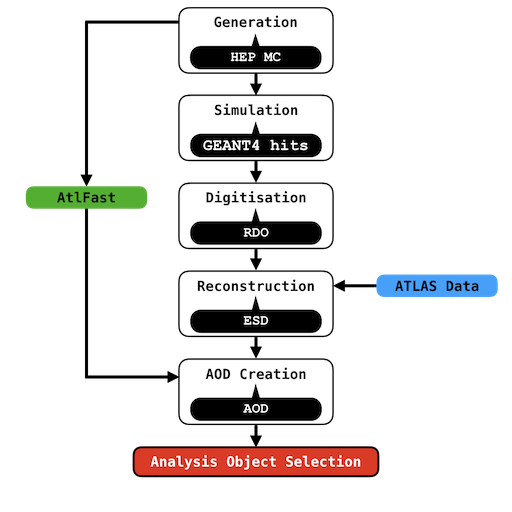
\includegraphics[width=.6\textwidth]{MCobj/flow}
		\caption{\label{fig:workflow} Illustration of the different stages of the work flow needed to produce analysable simulated and collected data outputs. The white boxes represent the processes, and their outputs are shown in black balloons: \ac{RDO}, \ac{ESD}, and the final product, \ac{AOD}. The green `AtlFast' box represents the alternative simulation method \textsc{Atlfast}~\cite{Lukas2012}, discussed in Section~\ref{subsec:detSim}. Finally, the blue box shows the stage at which the actual \ac{ATLAS} data events begin processing.}
	\end{figure}



	\section{Generation of an MC-simulated event}
	\label{sec:evGen}

		\ac{MC} event generators~\cite{Buckley:2011ms} are extensively used in particle physics to simulate \ac{SM} and \ac{BSM} physics processes. A combination of perturbative and phenomenological calculations, to produce randomly distributed physics events, of a given type, with stable final state particles, is employed. As already mentioned in Chapter~\ref{ch:detector}, The \ac{ATLAS} detector collects \pp- and heavy-ion-collisions data. When two protons collide at such high energy in the centre of mass, the collision essentially occurs between the nucleon constituents: partons\footnote{``\emph{Feynman~\cite{PhysRevLett.23.1415} interpreted the Bjorken scaling as the point-like nature of the nucleon's constituents when they were incoherently scattered by the incident electron. Feynman named the point-like constituents partons. This is the parton model.}''(taken from~\cite{Yan:2014kna})}. Three valence quarks (uud), the gluons mediating the strong interactions between the valence quarks, and the sea quarks produced in virtual \qqbar\ pairs due to interacting gluons, are included in the partons. Figure~\ref{fig:DIS} shows one of these interactions which are known as \ac{DIS} processes, simply because the substructure of the proton is probed, therefore \emph{deep}, by an incoming particle, in this case a proton, whose momentum is not conserved in the process, therefore \emph{inelastic}.

		\begin{figure}[!htb]
			\centering
			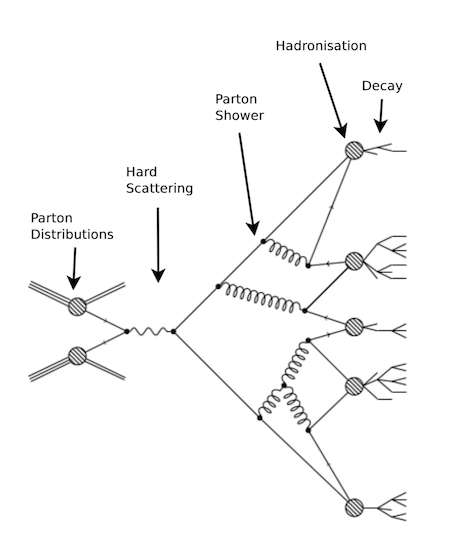
\includegraphics[width=.5\textwidth]{MCobj/ppcollision}
			\caption{\label{fig:DIS} Example of a \pp\ \ac{DIS} event.}
		\end{figure}

		An important, yet simplifying, dimensionless physical quantity is the Bjorken scaling~\cite{PhysRev.179.1547}, which represents the fraction, $x$, of the proton momentum carried by an interacting parton. The measure of momentum transfer $Q^2$ in such events, is related to the momentum transferred by the exchanged boson $q$ by $Q^2 = -q^2$. \acp{PDF} are used to describe mathematically the parton content of the colliding protons in order to model their interaction.  

		The \pp\ scattering at the \ac{LHC} can be categorised in processes such as \emph{hard}, which can be described with perturbation theory, or \emph{soft}, which involve non-perturbative \ac{QCD} effects. Typically, a \pp\ collision involves a hard scattering process between two partons, one for each proton, and a certain number of soft processes, such as \ac{ISR}, \ac{FSR}, and \ac{UE}. The \ac{ISR} involves particles, that are radiated by partons, which will interact in the hard process prior to their scattering. Those partons, which are not involved in the hard scattering process, the so-called \emph{spectators}, form the \ac{UE}. The \ac{FSR} refers to particles that are radiated from the final state products of the hard scattering. Furthermore, \emph{parton showering} is a process in which particles in the event that have colour can radiate gluons and/or produce \qqbar\ pairs. Products of these showers will undergo the process of \emph{hadronisation} during which colourless hadron states are produced if $Q^2$ is of the order of $1 \GeV$. Such a process occurs due to confinement. 

		%The modelling of the hard process, parton showering and hadronisation within the event, will be briefly described in Sections~\ref{sec:ME},~\ref{sec:PS} and~\ref{sec:hadronisation}. Section~\ref{sec:UE} describes how to model of the UE. 
		In order to allow analysers to select samples with relevant processes, \ac{MC} samples are divided in categories depending upon the hard-process specified before generation. It is also possible to filter events to only produce a given final state, \eg\ asking for zero leptons, in order not to waste computational resources on events which would not pass any selection criteria, regardless, improving the available statistics. The effect of the selection will be taken into account by applying filter efficiency when the analysis is carried out. The \textsc{HepMC} format is used to store the output of simulated data outputs~\cite{DOBBS200141}.

		\subsection*{Parton Distribution Function}
		%\label{sec:pdf}

			\acp{PDF}~\cite{Campbell2007} mathematically describe the probability density of constituent partons of the interacting protons to have a fraction, $x$, of the nucleon momentum. They depend upon the parton type such as, valence quark, gluon, or sea quark, and the momentum transfer $Q^2$. Although perturbative calculations of the \acp{PDF} are not feasible, the \textsc{DGLAP}~\cite{Gribov:1972ri, Altarelli:1977zs} evolution equations, using a range of hard scattering data from both fixed target and collider experiments, can be used to estimate the dependence as a function of $Q^2$ for a given parton. In other words, \acp{PDF} describe the evolution of the structure functions of quarks and gluons as a function of the running\footnote{Referred to a dependence on $Q^2$} strong coupling constant $\alpha_s$. Figure~\ref{fig:HERAPDF} shows the \acp{PDF}, calculated with input from \textsc{HERA} and \textsc{CTEQ} at $Q^2 = 10 \GeV^2$ for up and down valence quarks, gluons, and sea-quarks.

			\begin{figure}[!htb]
				\centering
				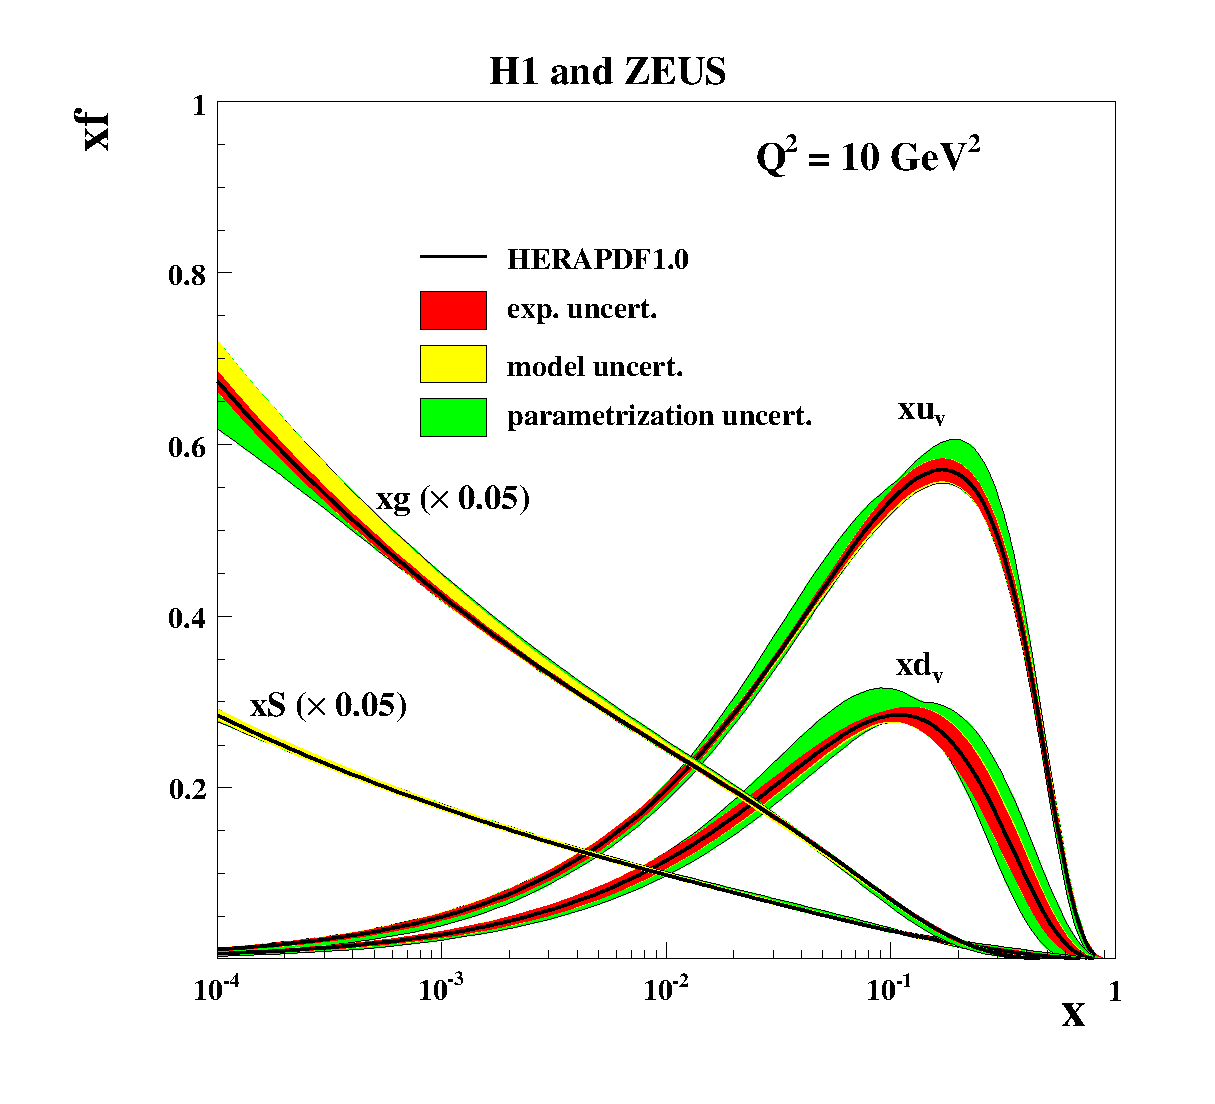
\includegraphics[width=.5\textwidth]{MCobj/d09-158f18b}
				\caption{\label{fig:HERAPDF} PDF from \textsc{HERAPDF1.0}, for up and down valence quarks $xu_v$ and $xd_v$ , gluons $xg$, and sea quarks $xS = 2x(\bar{U} + \bar{D})$, using a momentum transfer of $Q^2 =10 \GeV^2$ (from~\cite{Aaron:2009aa}).}
			\end{figure}

		\subsection*{Matrix Element}
		%\label{sec:ME}

			The matrix element is a simulation stage used to compute the hard processes, where a large momentum transfer ($Q^2 > \mathcal{O}(1 \GeV)$) is involved, which can be calculated using quantum field theory techniques. Matrix elements to \ac{LO} or \ac{NLO} in an expansion in $\alpha_s$, to calculate a probabilistic distribution of the outgoing partons, are used to make \acp{PDF} simulate partons coming into the hard scatter process. Hard emissions, namely the production of high momentum quarks and gluons in the event, therefore processes such as, a gluon splitting into two gluons, $g \to gg$, or a gluon decaying to a quark-antiquark pair $g \to \qqbar$, and a quark radiating a gluon ($q \to gq$), can be added into the matrix element.

		\subsection*{Parton Showers}
		%\label{sec:PS}

			The emission of extra soft objects cannot be modelled with the matrix element, due to its non-perturbative nature. \ac{PS} generators are instead used to include processes such as the emission of a gluon by a quark ($q \to qg$), or the emission of \qqbar\ pairs $g \to qq$ or a gluon pair by a gluon $g \to gg$. \textsc{Herwig}~\cite{Herwig2001}, \textsc{Pythia}~\cite{Pythia2006}, and \textsc{Sherpa}~\cite{Sherpa} collaborations have developed the most used \ac{PS} models across the \ac{ATLAS} community and beyond. Markov chains~\cite{Berg2004} are the heart of the algorithms used to simulate \ac{PS}. These use probabilities that a gluon is radiated or a \qqbar\ pair is produced. %The decision of whether or not these processes will occur is made at each point in the chain. 

			At intermediate $Q^2$, gluon/quark radiation may be treated as a hard emission or part of the \ac{PS}, meaning that, in a given event double-counting might occur. To overcome such issue, the \ac{CKKW}~\cite{QCD2001}, and the \ac{MLM}~\cite{ME2001}, schemes are employed to determine whether the emissions are part of the matrix element or \ac{PS}. As the energy of the partons decrease below $1 \GeV$ they will undergo hadronisation.

		\subsection*{Hadronisation}
		%\label{sec:hadronisation}

			As previously mentioned in Section~\ref{sec:SMov}, once the quarks and gluons in the final state reach a $Q^2$ of the order of $\Lambda_{\mathrm{QCD}} \sim 200 \MeV$, the recombination into colourless objects must occur. The modelling of the production of such bound state, the hadronisation, involves non-perturbative \ac{QCD} and many more parameters than the parton showering. Phenomenological models, tuned using data, are then needed. The cluster model~\cite{ClusterHerwig1999}, used by \textsc{Herwig}, and the Lund string model~\cite{LundModel2002}, used by \textsc{Pythia}, are the most employed. 

		\subsection*{Underlying Event}
		%\label{sec:UE}

			Partons not involved in the hard process of the event, referred to as the \ac{UE}~\cite{Field2008}, can lead to a certain number of soft interactions at a lower energy scale, therefore producing additional hadronic activity in the event. Once again, phenomenological models are used to account for such effect which is modelled within \textsc{Sherpa} and \textsc{Pythia} where a whole lot of additional free tuned-to-data parameters are included. More details can be found in~\cite{Field2008}.

		\subsection*{Detector simulation}
		\label{subsec:detSim}

			Although at this stage the output of the \ac{MC} generators contains all the kinematic features of the event, it is not yet possible to compare to the \ac{ATLAS} collected data, as the interactions of the particles passing through the detectors are not yet included. The \textsc{Geant4} software~\cite{Geant42003}, included within the \ac{ATLAS} offline software\footnote{All the software made available for analysers to be used after the data have been collected}, is used to simulate the energy deposited within the detector: a first stage is run to simulate the interactions of the particles with the various sub-systems, and a second one is run to convert energy deposits into detector-output-like signals (voltage, times, etc.). This is the so-called \emph{digitisation}. The output is now produced with a format that is identical to the one produced by the \ac{ATLAS} \ac{TDAQ} system, therefore \ac{MC} and collected \ac{ATLAS} data can now be consistently processed by the same trigger and reconstruction software. Nonetheless, the \ac{ATLAS} Collaboration also use faster simulation software such as \textsc{Atlfast-II} (AF2)~\cite{Lukas2012} where, in order to reduce the usage of the available computational resources, a parametrised description of the showers in the calorimeters is implemented. 


	\section{Object Reconstruction}
	\label{sec:objReco}

		At this stage both \ac{MC} and data samples contain all the electronic pulses from the digitisation process. These have to be turned into tracks and calorimeter deposits which, in turn, have to processed to be reconstructed into physics object, such as electrons, photons, muons, jets, taus, and missing energy, \met. Initially, a set of loose definitions is employed in order for various analyses to use such objects. Later, a set of tighter cuts can be applied depending on what a particular analysis needs to focus on. This approach increases the purity of the selected objects at the expense of selection efficiency. The criteria used to define the physics objects, relevant to the analysis presented in this thesis, will be presented in the following paragraphs.


		\subsection*{Tracks and vertices}

			When a charged particle passes through the detector, all the \ac{ID} sub-systems, pixel, \ac{SCT} and \ac{TRT} components, register ``hits''and then, tracing the particle's trajectory, the hits are reconstructed into a ``track''. The most used algorithm is the so-called \emph{inside-out} method, whose clue is in the name: it works outwards from the centre of the \ac{ID} to produce a track once it has initially grouped together hits in the pixel and \ac{SCT} sub-systems. If this track is then compatible with hits in the \ac{TRT} detector, then these hits are also included and the track is accepted. On the contrary, the back-tracking algorithm tries to reconstruct a track starting from the \ac{TRT} to the \ac{SCT} and Pixel detectors. Tracks can also be reconstructed using only the hits in the \ac{TRT}. A number of selection cuts are applied to the tracks in order to achieve the required quality. Signals produced in other parts of the detector are then used to match \ac{ID} tracks up with charged-particle candidates, \eg\ \ac{ECAL} cluster for an electron track. The $\eta$ and $\phi$ values are then assigned to tracks using their direction with respect to the origin\footnote{This is assumed to be the position of the primary interaction} in the co-ordinate system described in Section~\ref{par:coord}. The relation that links the \pt\ of a track to its bending radius and the magnetic field is $\pt = 0.3 \times B \times R$, where the \pt\ is given in \GeV, the magnetic field $B$ in Tesla, and the radius $R$ in meters. Moreover a set of variable is defined:

			\begin{itemize}
				\item $d_0$ : the distance of closest approach between the track and the origin
				\item $z_0$ : the $z$-plane component of $d_0$;
				\item $z_0 \sin \theta$ : the projection of $d_0$ onto the $z$-axis
			\end{itemize}

			Vertex reconstruction is needed for various purposes \eg\ to differentiate objects from the interesting hard scattering from other pile-up interactions. As the bunch length is finite, \pp\ interactions are spread out along the $z$ coordinate. In order to reconstruct the \ac{PV}, tracks are back-tracked to the beam line. Table~\ref{tab:tracksCuts} shows a set of cuts applied to the reconstructed \ac{ID} tracks to be used for vertex reconstruction.

			\begin{table}[!htb]\centering\caption{Cuts applied to the tracks}							
				\begin{tabular}{|cc|}
					\hline \hline
					\textbf{Variable} & \textbf{Cut} \\ \hline \hline
					\pt & $> 400 \MeV$ \\
					$\abseta$ & $< 2.5$ \\ 
					\# \ac{IBL} hits + B Layer hits & $\geq 1$ \\ 
					\# shared modules\footnotemark & $\leq 1$ \\
					\# Pixel holes\footnotemark & $== 0$ \\
					\# \ac{SCT} holes & $\leq 1$ \\ \hline
					\multirow{2}{*}{\# Si\footnotemark hits} & $\geq 9$ if $\abseta \leq 1.65$ \\
									&  $\geq 11$ if $\abseta > 1.65$ \\ 
					\hline \hline
				\end{tabular}

			\label{tab:tracksCuts} 
			\end{table}
			\footnotetext{$1$ shared Pixel hit or $2$ shared \ac{SCT} hits}
			\footnotetext{Holes exist when a hit is expected in a layer of sensors given the fitted trajectory of the track but none is found}
			\footnotetext{\emph{Silicon} refers to IBL, Pixel and SCT}

			A global maximum in the $z$ coordinate of reconstructed tracks is searched for first, to find a vertex seed. The vertex position is then fitted using an algorithm called the \emph{Adaptive Vertex Fitting} algorithm~\cite{ATL-PHYS-PUB-2015-026,Fruhwirth:2007hz}. The vertex position is determined by fitting to \ac{ID} tracks with the least squares fitting method. Outlier tracks\footnote{Tracks that are far from the vertex centre} are assigned lower weights in the fit than tracks close to the vertex centre. Outlier tracks have a high probability of being tracks that not originating from another vertex. 
			The adaptive fitting algorithm is able to decrease the sensitivity to these tracks by applying a smaller weight. As we do not know a priori the true position of the vertex centre, and which tracks are outliers, the algorithm iteratively tries to fit the vertex: all tracks weights are initialised with high values; after each fit iteration the weight of the outlier tracks is decreased; the algorithm then determines both the vertex centre and which tracks are outliers with increasing accuracy after each iteration; finally, the algorithm will stop once the fitted vertex centre does not change any more. Furthermore, once a vertex is found, tracks which are incompatible with the found vertex will form a new vertex seed. The vertex reconstruction process will terminate once all the tracks have been clustered into vertices or no additional vertices can be found. Among all the vertices found by the algorithm the \ac{PV} will be the one with the highest sum of the squared momenta of the associated tracks $\left ( \Sigma \pt^2 \right)$. The remaining primary vertices found by the algorithm, if any, are referred to as pile-up vertices. Further detail about the algorithm can be found in references~\cite{ATL-PHYS-PUB-2015-026,Fruhwirth:2007hz}. 

			Secondary vertices can also be reconstructed by looking at the displacement, with respect to the primary vertex position, due to the distance travelled by a decaying particle whose lifetime is sufficiently long for the decay length e.g. b-quarks, which travel a few millimetres.


		\subsection*{Electrons and Photons}

			Clusters of energy deposits in the electromagnetic calorimeter are used to reconstruct both electron and photon. The \ac{ECAL} is divided into a grid of towers, each of which measuring $\Delta \eta \times \Delta \phi = 0.025 \times 0.025$. The total tower energy is calculated summing the energy from all longitudinal layers inside each tower. A sliding-window algorithm groups energy towers into \ac{EM} clusters~\cite{ATL-PHYS-PUB-2016-015,Aad:2014nim}. The window width is $3 \times 7$ towers in the barrel and $5 \times 5$ towers in the endcap. The reconstructed cluster therefore has a size of $\Delta \eta \times \Delta \phi = 0.075 \times 0.175$ in the barrel and $0.125 \times 0.125$ in the endcap. In order to achieve better cancellation of systematics when using electrons to measure the photon response, the same window size is employed for electrons and photons~\cite{ATL-PHYS-PUB-2016-015}. Monte-Carlo-based algorithms and data-driven corrections, derived from \Zee\ events, are employed to carry out energy calibration~\cite{ATL-PHYS-PUB-2016-015}. Figure~\ref{fig:elRecoAlg} shows an illustration of the electron reconstruction algorithm.

			\begin{figure}[!htb]
				\centering
				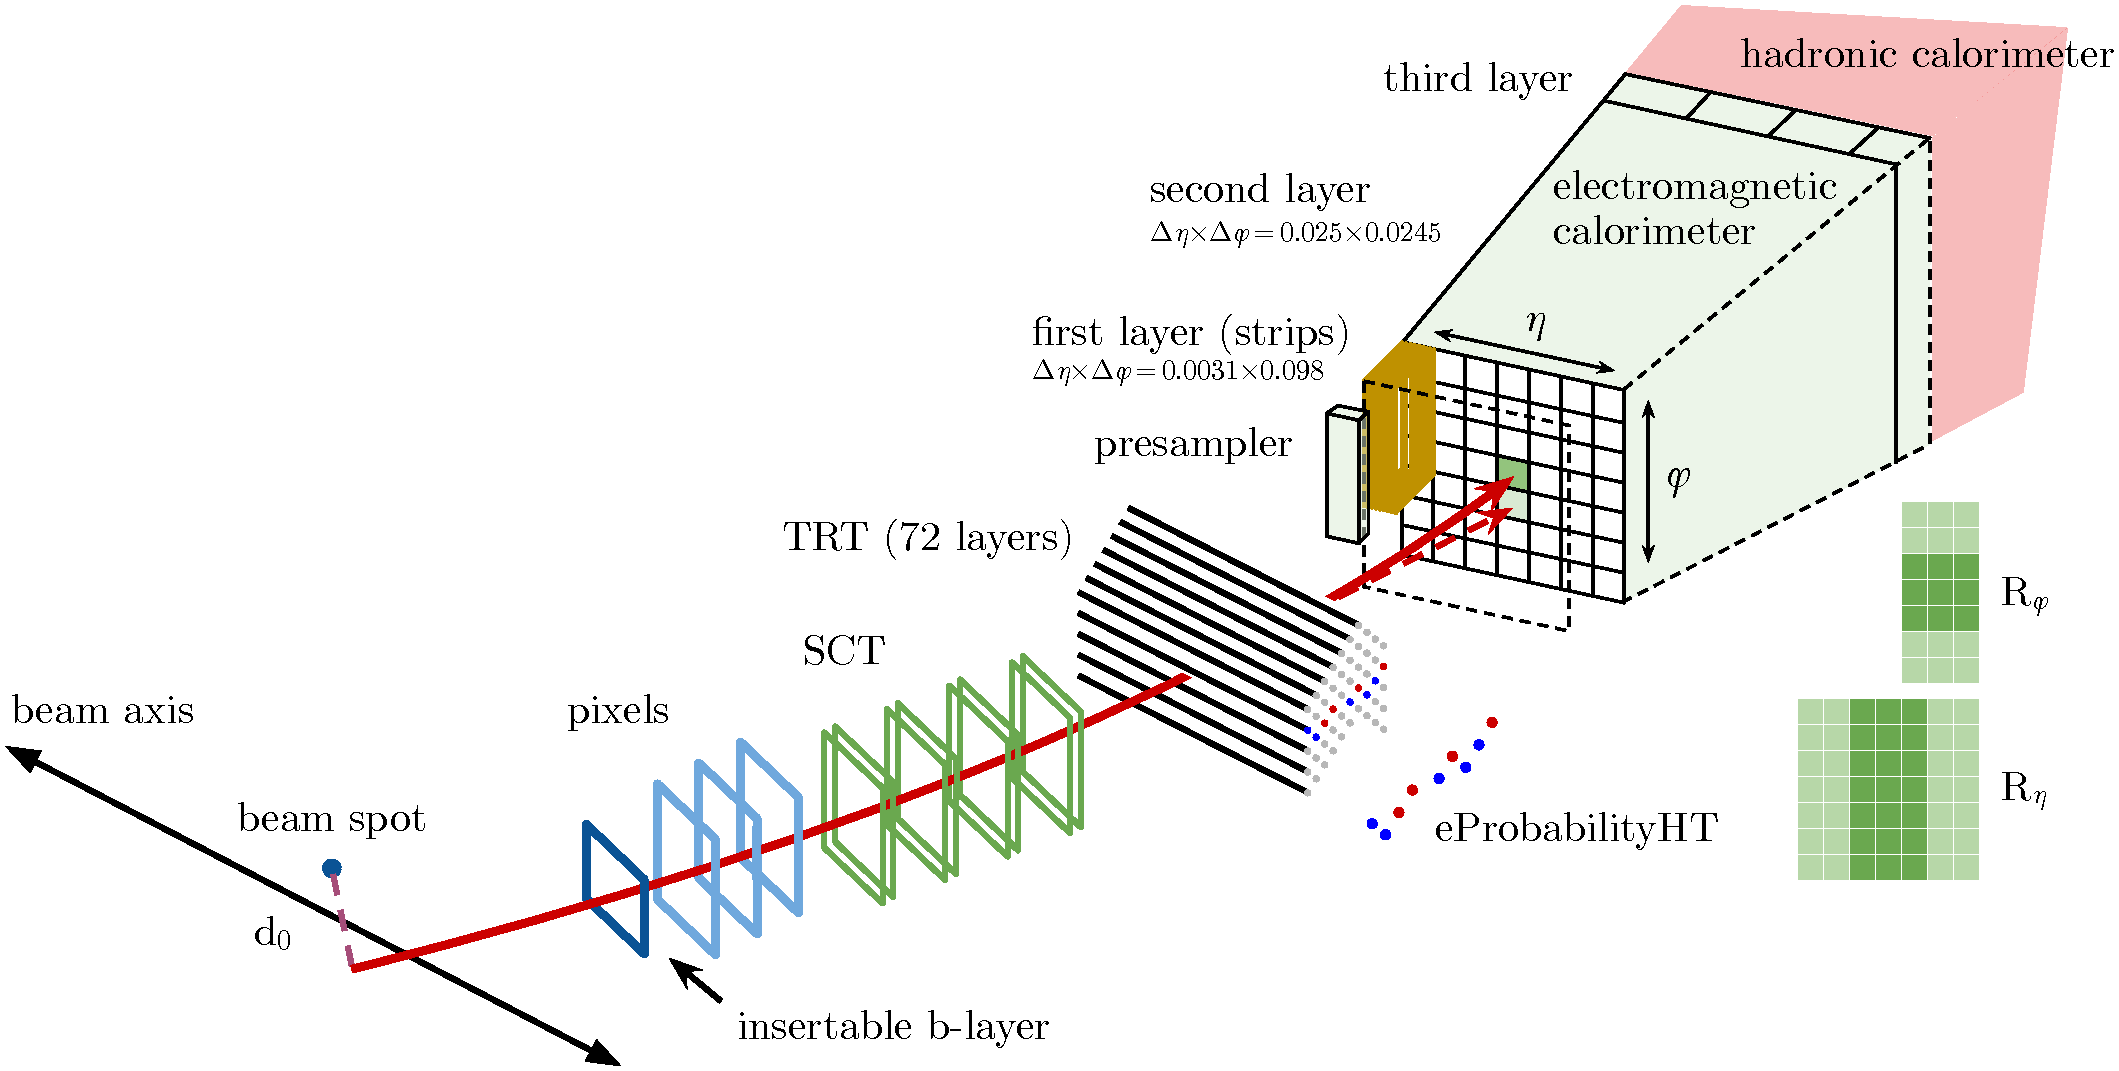
\includegraphics[width=\textwidth]{MCobj/elRecoAlg}
				\caption{\label{fig:elRecoAlg} Schematic view of the electron reconstruction and identification (taken from~\cite{ATLAS:2016iqc}).}
			\end{figure}

			Identified clusters are then matched to reconstructed \ac{ID} tracks (required to have a minimum number of pixel and silicon hits) using the track and cluster position. A cluster will be either considered as an electron or a photon candidate, if it satisfies one of the following criteria:

			\begin{description}
				\item \textbf{electron}: one single reconstructed \ac{ID} track with an associated vertex;
				\item \textbf{unconverted photon}: no \ac{ID} tracks;
				\item \textbf{converted photon}: two opposite-signed collinear tracks (consistent with electrons) are associated with a secondary vertex;
				\item \textbf{converted photon}: single track is present but there are missing hits in the \ac{IBL}
			\end{description}

			Once electrons and photons have been reconstructed an additional set of criteria is employed to rule out any potential misidentification. In particular, the identification is based on a \ac{LH} algorithm that depends on variables such as shower shape, radiation deposited in the \ac{TRT}, and associated-track properties. Identification \acp{WP}, such as \texttt{Loose}, \texttt{Medium} and \texttt{Tight}, are employed to identify electrons using different selections, which will reflect in different efficiencies and purities\footnote{The number of actual electrons (photons) among the selected candidates.}, as the tighter the identification is, the purer the selected object will be. Figure~\ref{fig:ElPhIDEff} shows the reconstruction and identification efficiencies using $2016$ data for electrons, and $2015+2016$ for unconverted photons. Here, the data-\ac{MC} discrepancy in the electron identification performance is due to a mismodelling of the \ac{TRT} conditions in addition to the known mismodelling of calorimeter shower shapes in the \textsc{Geant4} detector simulation~\cite{PubEGAMMA}. Nonetheless, scale factors\footnote{Calibration factors derived from data.} were derived and applied to the Monte Carlo, to match the performance observed in the data.

			\begin{figure}[!htb]
				\begin{center}
					\subfloat
						[Electron reconstruction and identification efficiencies in \Zee\ events as a function of \et, integrated over the full pseudo-rapidity range. The data efficiencies are obtained by applying data/MC efficiency ratios that were measured in \Jee\ and \Zee\ events to MC simulation. The total statistical and systematic uncertainty is shown.]
						{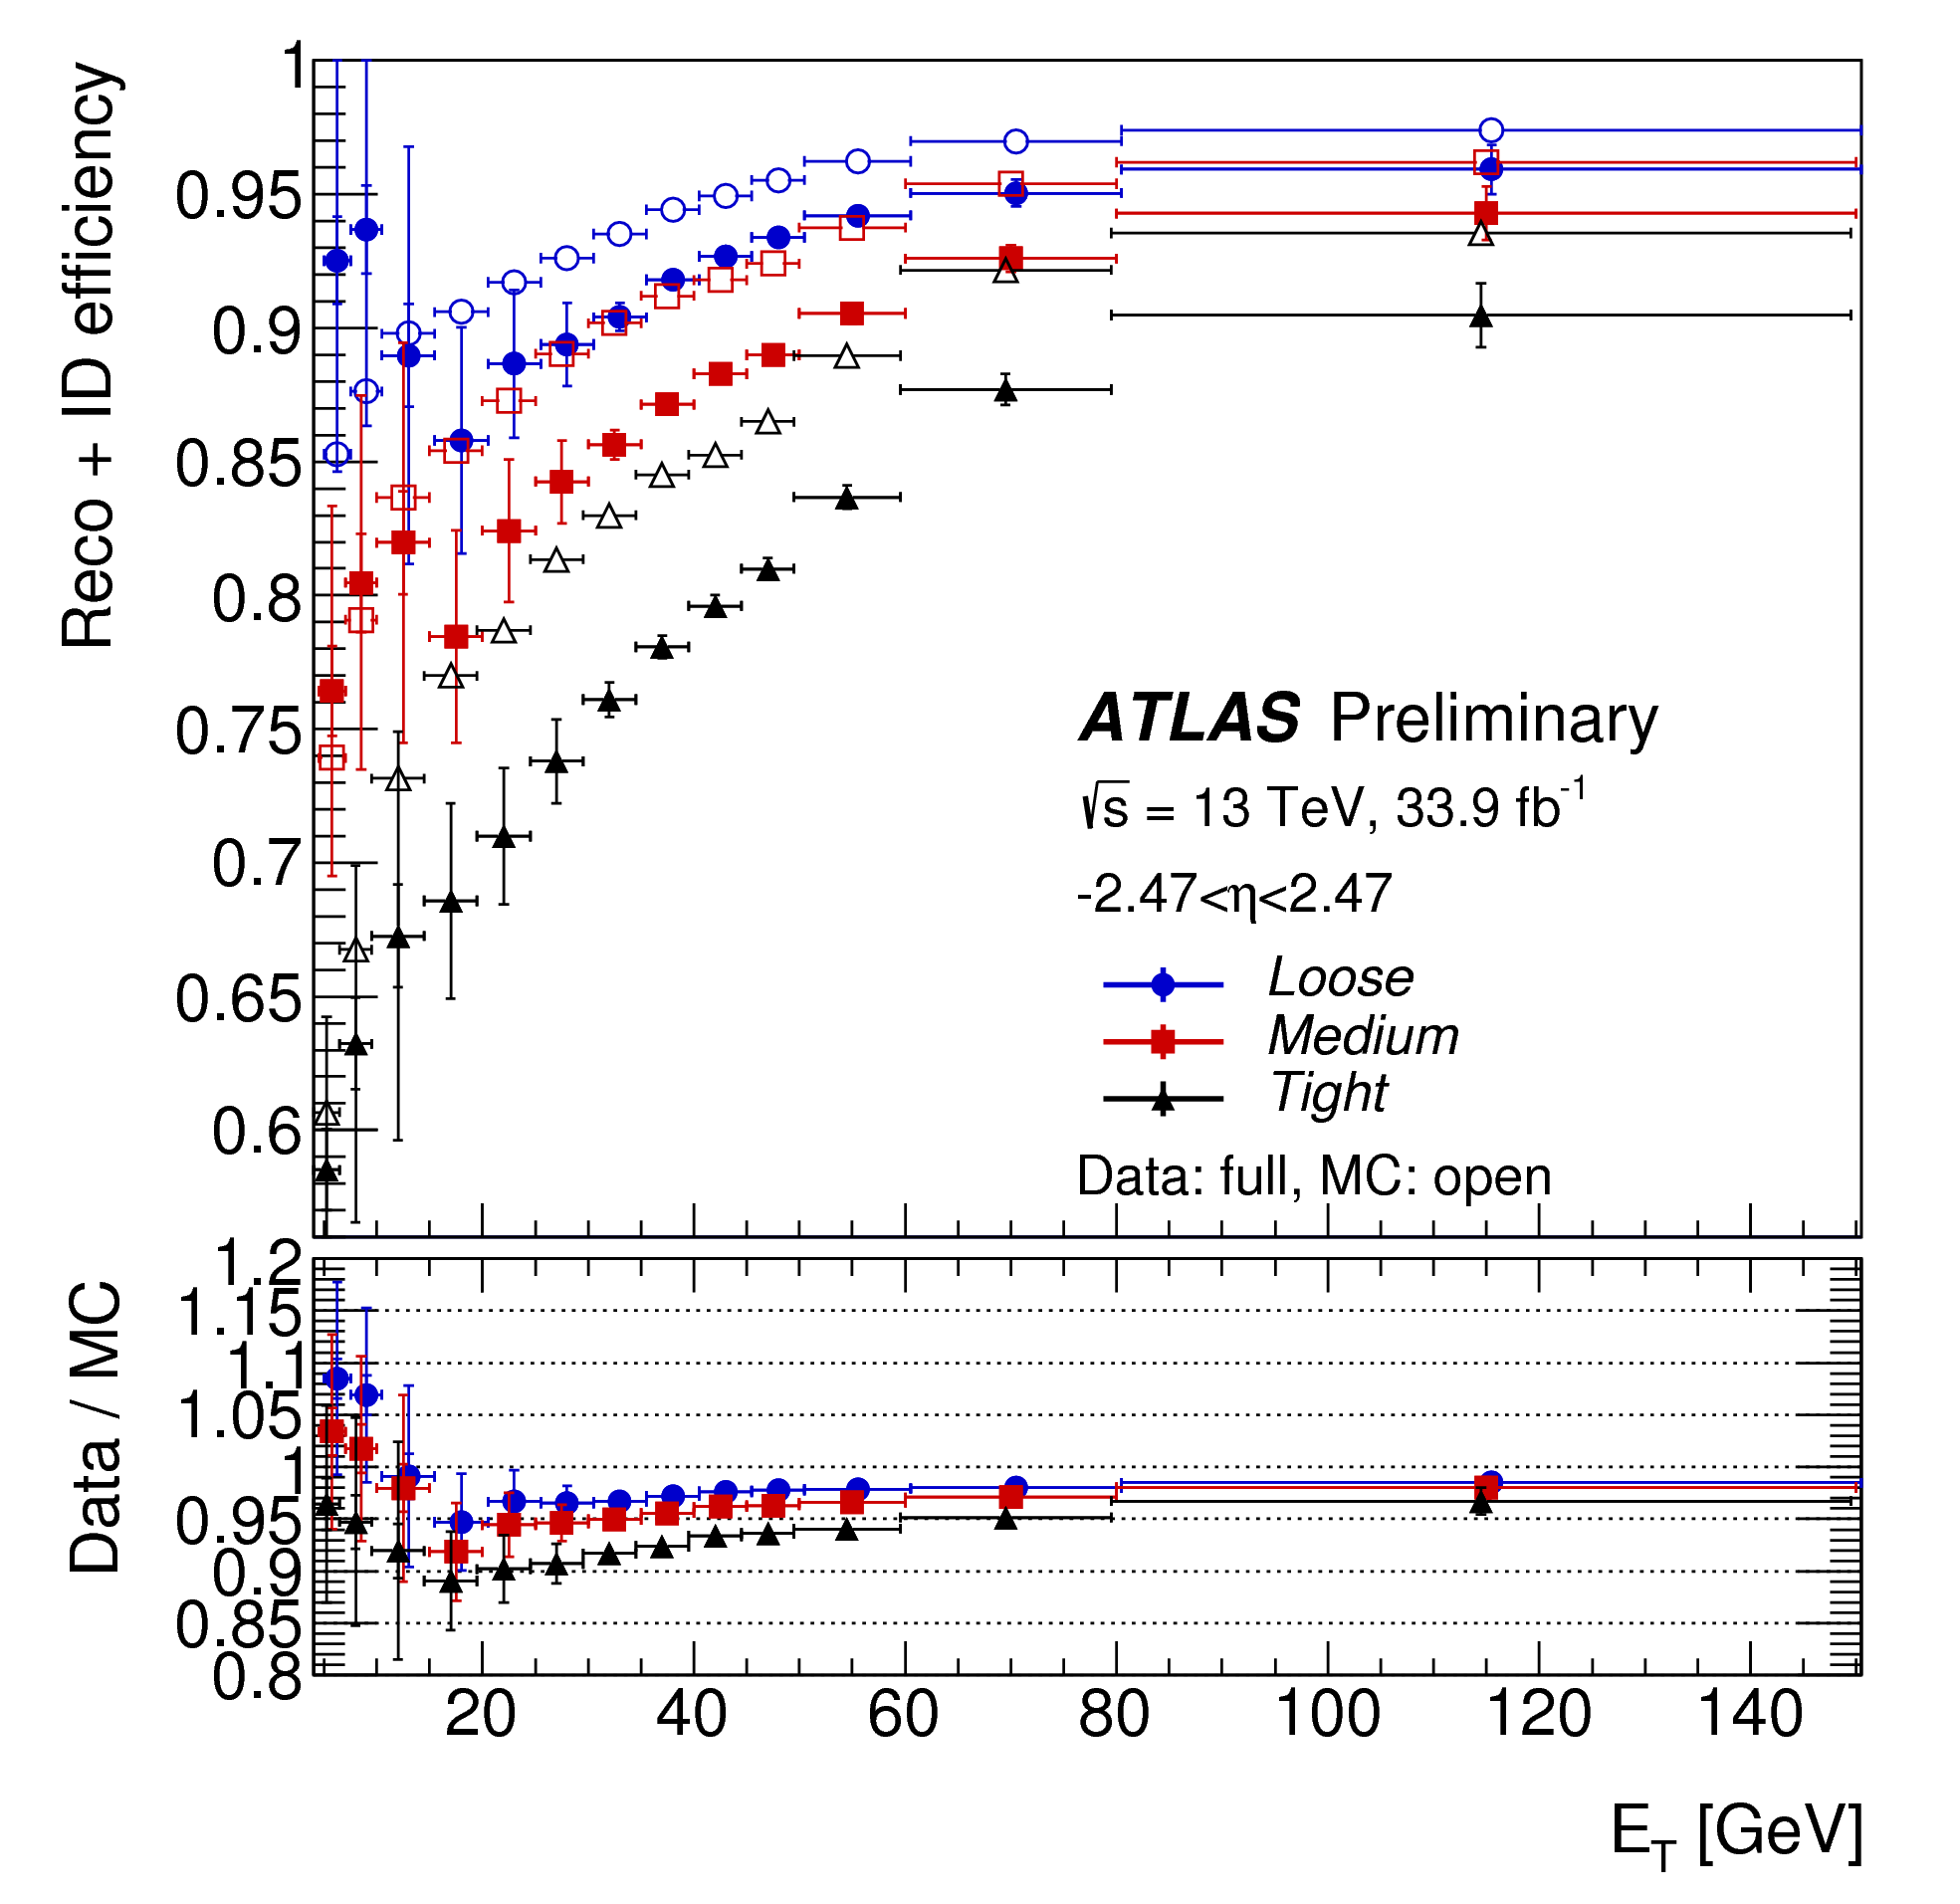
\includegraphics[width=0.4\textwidth]{MCobj/elRecoIDEff}}\hspace{0.05\textwidth}
					\subfloat
						[Photon identification efficiencies using the full $2015 + 2016$ dataset Comparison of the data-driven measurements (radiative \Zboson\ decay, electron extrapolation and matrix method~\cite{Aaboud:2016yuq}) of the identification efficiency for unconverted photons as a function of \et\ in the region $10 \GeV < \et < 1500 \GeV$ for the pseudo-rapidity interval $\abseta < 0.6$. The error bars represent the sum in quadrature of the statistical and systematic uncertainties estimated in each method.]
						{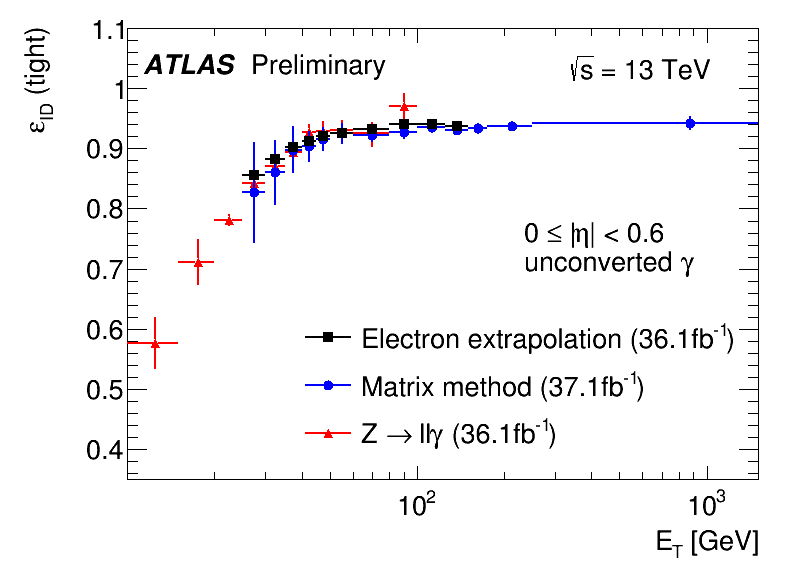
\includegraphics[width=0.5\textwidth]{MCobj/phRecoIDEff}}
				\end{center}
				\caption{Electron and photon reconstruction and identification efficiencies (taken from~\cite{PubEGAMMA}).}
				\label{fig:ElPhIDEff}
			\end{figure}

			The shower shape and the amount of hadronic activity behind the \ac{EM} cluster are at the heart of photon identification. The \ac{EM} showers originating from photons and those originating from neutral mesons \eg\ $\pi_0$ can be distinguished by looking at the energy deposited in the cells within the first and second layer of the \ac{ECAL}~\cite{ATL-PHYS-PUB-2016-014}. Two categories of photons are reconstructed employing two identification \acp{WP}: \texttt{Loose} and \texttt{Tight}. The former are typically used for triggering, the latter for physics analysis, such as the one presented in Chapter~\ref{ch:stop_ana}, where, the top-quark pair production in association with a photon, \ttgamma\ was studied.

		\subsection*{Muons}

			Two independent track fits in the \ac{ID} and \ac{MS} are the basis of the muons selection procedure. Depending on the signature in each sub-system the fits are combined using different algorithms. Various categories of muons can be reconstructed with the \ac{ATLAS} detector~\cite{Aad:2016jkr} and they can be listed as it follows: 

			\begin{description}
				\item \textbf{Combined:} candidates whose tracks are found in both \ac{ID} and \ac{MS} on which a global refit is run to obtain a combined muon track that describes the trajectory of the particle through the whole detector, in order to take into account the energy loss in the calorimeter;

				\item \textbf{Extrapolated:} candidates in the forward region ($2.5 < |\eta| < 2.7$) that produced a track in the \ac{MS} but fell outside the \ac{ID} acceptance, therefore their trajectory is reconstructed using the \ac{MS} track, loosening its compatibility requirement with the interaction point;

				\item \textbf{Segment tagged:} candidates whose tracks in the \ac{ID} are found to have a corresponding hit in the inner layer of the \ac{MS}. Generally for muons with low \pt\ or due to cracks in the \ac{MS};

				\item \textbf{Calorimeter tagged:} candidates, whose \ac{ID} tracks can be matched with an energy deposit in the calorimeter, compatible with the signature of a \ac{MIP}, with no associated \ac{MS} tracks; mainly muons in the central pseudo-rapidity region ($|\eta| < 0.1$) due to a crack in the barrel of the \ac{MS};
			\end{description}

			\begin{figure}[!htb]
				\begin{center}
					\subfloat
						[Muon reconstruction efficiencies for the \texttt{Medium} identification algorithm measured in \Jmm\ and \Zmm\ events as a function of the muon \pt. The prediction by the detector simulation is depicted as empty circles (squares), while the full circles (squares) indicate the observation in collision data for \Jmm\ (\Zmm) events. Only statistical errors are shown in the top panel. The bottom panel reports the efficiency scale factors. The darker error bands indicate the statistical uncertainty, while the lighter bands indicate the quadratic sum of statistical and systematic uncertainties.]
						{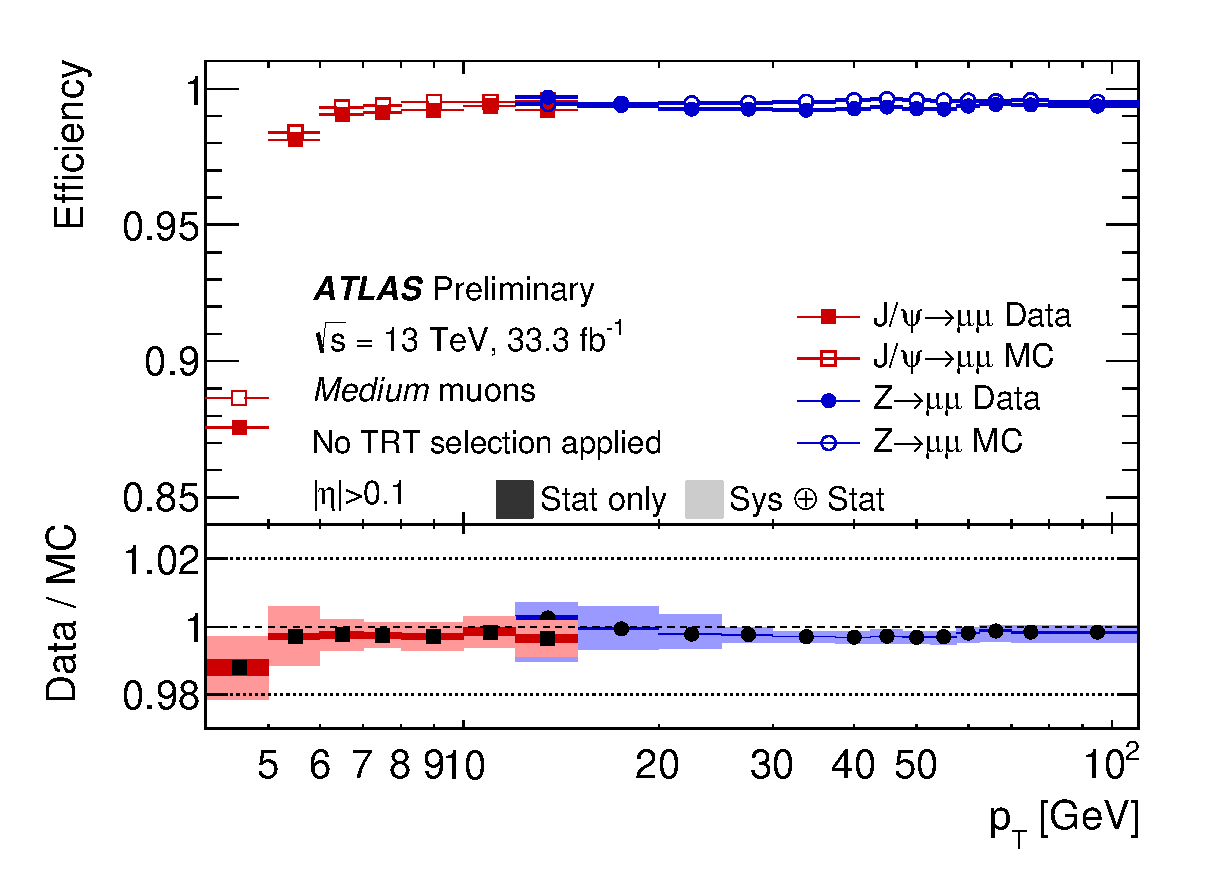
\includegraphics[width=0.45\textwidth]{MCobj/muRecoIDEff_pt}}\hspace{0.05\textwidth}
					\subfloat
						[Muon reconstruction efficiencies for the \texttt{Loose/Medium/Tight} identification algorithms measured in \Zmm\ events as a function of the muon $\eta$ for muons with $\pt > 10 \GeV$. The prediction by the detector simulation is depicted as open circles, while filled dots indicate the observation in collision data with statistical errors. The bottom panel shows the ratio between expected and observed efficiencies, the efficiency scale factor. The errors in the bottom panel show the quadratic sum of statistical and systematic uncertainty.]
						{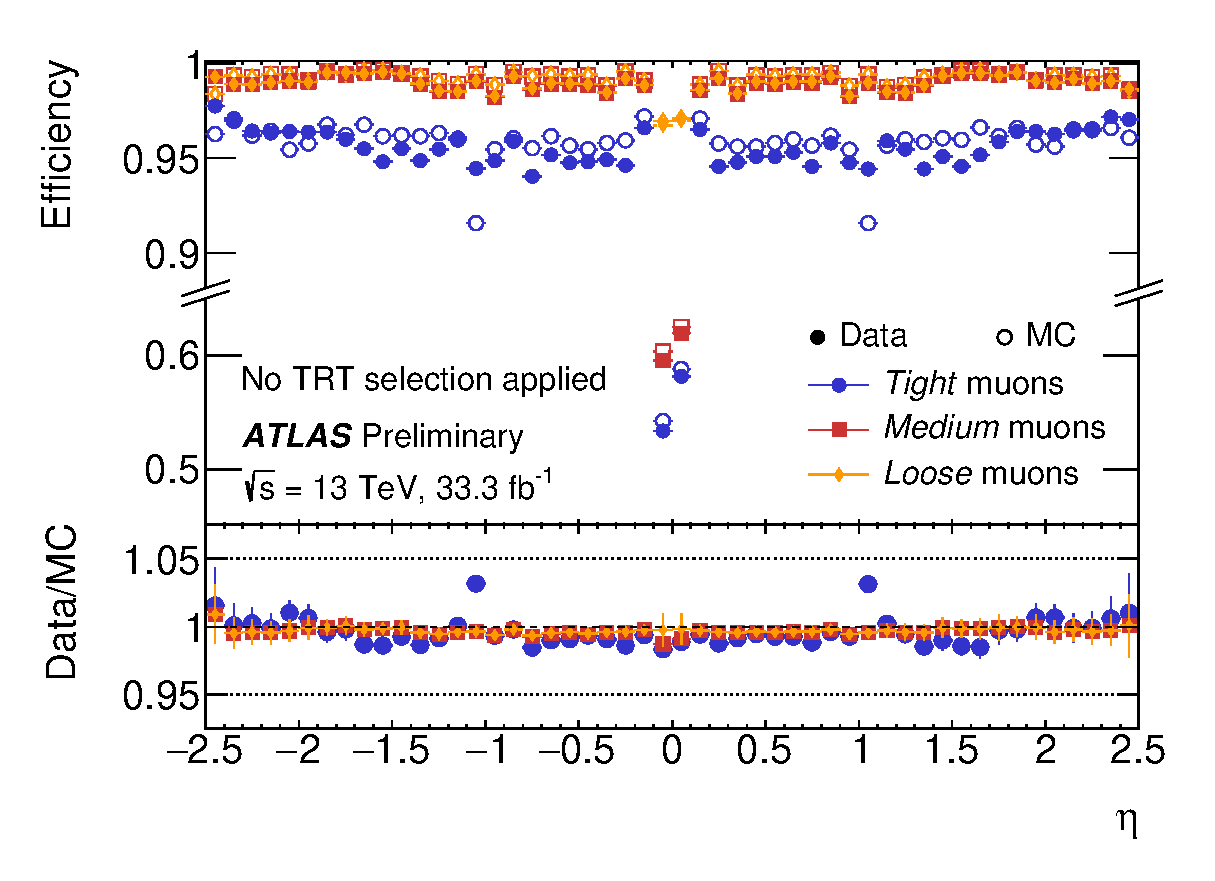
\includegraphics[width=0.45\textwidth]{MCobj/muRecoIDEff_eta}}
				\end{center}
				\caption{Muon reconstruction and identification efficiencies (taken from~\cite{PubMuons}).}
				\label{fig:MuIDEff}
			\end{figure}

			In order to separate prompt muons from backgrounds such as pions and kaons decays, further identification requirements are employed, \eg\ track quality requirements in the \ac{ID} and the \ac{MS}, normalised $\chi^2$ of the combined track fit, etc.). 

			Figure~\ref{fig:MuIDEff} shows reconstruction and identification efficiencies as a function of \pt\ and $\eta$. Likewise electrons and photons, in order to meet all the different requirements of the various \ac{ATLAS} analyses, a set of \acp{WP} is defined. The performance is calibrated using the so-called tag-and-probe method\footnote{Method used to select, from known resonances such as \Zee\, unbiased samples of electrons (probes) by using strict selection requirements on the second object produced from the particle’s decay (tags)~\cite{EleReco2011}.} in \Zmm\ or \Jmm\ events. Further details can be found at~\cite{Aad:2016jkr}.


		\subsection*{Jets}

			As already mentioned in Sections~\ref{sec:SMov} and~\ref{sec:evGen}, due to \ac{QCD} confinement when a \pp\ collision occurs, a spray of hadronic matter, or \emph{jet}, is produced. A jet in the \ac{ATLAS} detector looks like an object that released its energy in both \ac{ECAL} and \ac{HCAL} via \ac{EM} and hadronic showers and, as it is generally comprised of a certain number of charged particles, it also has \ac{ID} tracks associated with the showers. The identification and the reconstruction of jets is important for the analysis discussed in Chapter~\ref{ch:stop_ana}, which targets the $pp \to \stop \bar{\stop} \to bqq \ninoone + \bar{b}\bar{q}\bar{q} \ninoone$ channel where all the visible decay products are quarks, therefore jets. A brief description of jet reconstruction and calibration is presented in the following paragraphs.

			%\paragraph*{Reconstruction}

				The three-dimensional structure of topological clusters in the calorimeters is used to measure the energy deposited by the showers through the clusters\cite{LamplAlgo2008,Aad:2016upy}. These are built up via an iterative algorithm which first forms the core of the cluster by identifying seed cells, with a high energy threshold, and adding adjacent cells with a lower threshold, and then, in order to account any potential shower leak an extra layer of cells is added, such that a collection of topological clusters per event is obtained. Jet-finding algorithms, which treat jets as massless objects, are then fed with such clusters information such as energy and position. The former is calculated as the sum of all the energy deposits in the cells previously identified, whose position within the detector is used to deduct angular information. A widely used algorithm within the \ac{ATLAS} Collaboration is the \antikt\ one which forms a collection of jets as output by iteratively recombining the input clusters. The algorithm essentially groups two object into a single one according to a distance $d_{ij}$, defined as: 

				\begin{equation}
					d_{ij} = \min \left ( k_{t_{i}}^{2p}, k_{t_{j}}^{2p}\right ) \frac{\Delta_{ij}^2}{R^2}
				\label{eq:dij}
				\end{equation}
				
				\noindent where $i$ and $j$ are topological cluster indices, $k_t$ is the transverse momentum of each topological cluster, $\Delta_{ij}^2 = \Delta \phi_{ij}^2 + \Delta \eta_{ij}^2 $ is the distance between the two topological clusters, and $R$ is an input parameter into the algorithm which, in the analysis presented in this work, is set to $R = 0.4$. The topological clusters $i$ and $j$ which minimise $d_{ij}$ are then combined to form larger individual clusters. The next iteration takes into account the larger individual clusters as well as the remaining initial topological clusters and combines them according to the same procedure, which is repeated until all remaining topological-cluster pairs satisfy $\Delta_{ij}> R$. Additional information can be found at~\cite{Antikt2008}.

			%\paragraph*{Calibration}

				Due to the compensation condition\footnote{Calorimeters response can be described in terms of the \ac{EM}/Hadronic ratio, as it is a measure of the calorimeter response to \ac{EM} VS hadronic radiation. An ideal calorimeter would have \ac{EM}/Hadronic$\sim1$.} the hadronic component of the shower produced by jets is underestimated and for such reason a calibration procedure is employed. In particular, the so-called Electromagnetic + Jet Energy Scale scheme is employed~\cite{ATL-PHYS-PUB-2015-015} where a set of corrections is applied to match the energy of the initial partons. These are \textbf{vertex correction}: once the \antikt\ algorithm has reconstructed the jets, its four-vectors, initially pointing at the centre of the detector, are adjusted to point to the primary vertex; \textbf{pileup correction}: pileup effect on the jets energy is reduced by using an area-based subtraction procedure~\cite{TheATLAScollaboration:2013pia}; \textbf{jet energy and $\eta$ correction:} additional calibration based on energy and pseudo-rapidity corrections where the kinematical properties of the reconstructed jet (\pt\ and $\eta$) are compared to the ones derived from \ac{MC} simulations; \textbf{global sequential correction:} individual jet property-based correction for properties such as the fraction of energy deposited in different calorimeter layers or the number and type of associated tracks~\cite{ATLAS:2015oia}; \textbf{in-situ corrections:} then measured \pt\ of the jet is corrected using multi-jet and $\gamma$/\Zboson+jets events, where the momentum of a \emph{probe} jet is balanced against a well-measured reference object~\cite{ATLAS-CONF-2015-017}.

			Finally, the \ac{JVT} variable~\cite{ATLAS-CONF-2014-018}, related to the fraction of charged tracks within the jets that point to the primary vertex, is employed. This observable tests the compatibility between the reconstructed jet and the hard-scatter charged particles within the jet~\cite{Aaboud:2017pou}.


		\subsection*{$b$-tagged jets}

			The identification and the reconstruction of jets originated from $b$-quarks is also important, as they also are part of the final state of the analysis presented in this work. Not only is this crucial for this work but also for other analyses carried out by the \ac{ATLAS} Collaboration. The standard jet-reconstruction procedure discussed above applies to \bjs\, too, with the addition of dedicated algorithms ($b$-tagging~\cite{Aad:2015ydr}) employed to spot a $b$-hadron within their cone. A diagram, showing the difference between light jets and \bjs\, is shown in Figure~\ref{fig:btagpic}. Due to their lifetime ($\sim 10^{-12}$ s), $b$-hadrons can travel a measurable distance in the detector before decaying ($\sim 1$ mm for a $20$-\GeV\ \bj), therefore producing a \ac{SV} which, together with a requirement on the impact parameter $d_0$, already provides a useful discrimination tool for jet flavour. Unfortunately, \cjs\ also leave a similar signature within the ATLAS detector. Although on average they travel a shorter distance due to their shorter lifetime~\cite{ATL-PHYS-PUB-2015-001}, their presence introduces a source of background for $b$-tagging. 

			\begin{figure}[!htb]
				\centering
				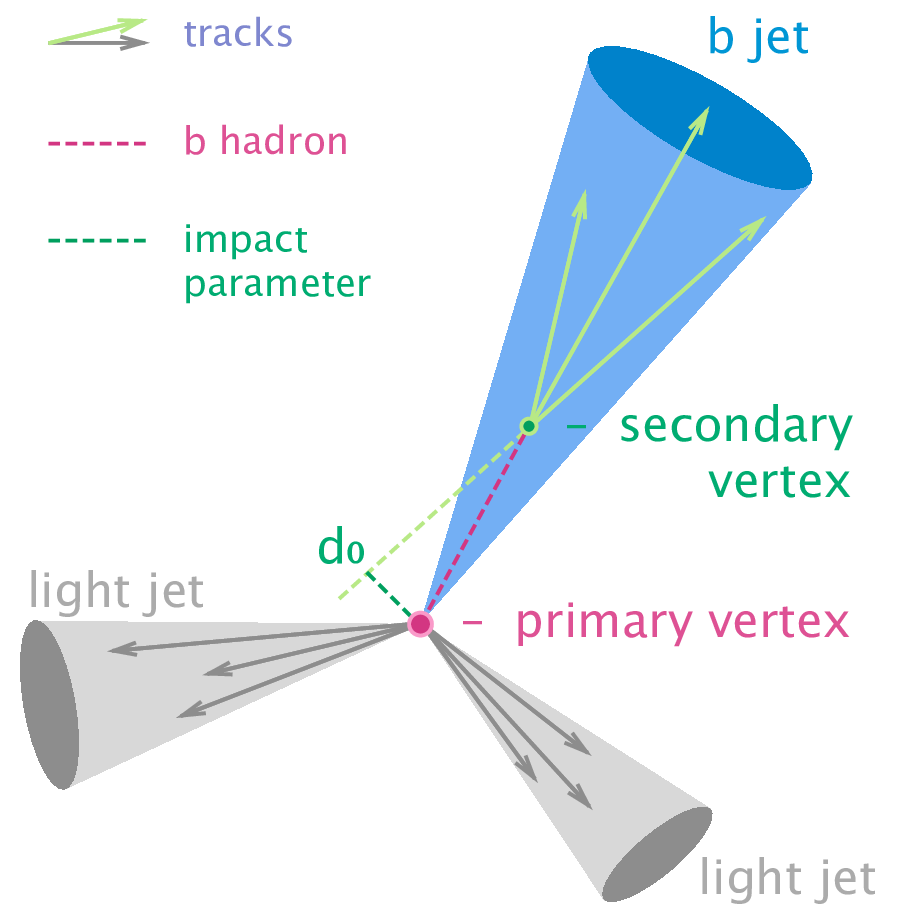
\includegraphics[width=.5\textwidth]{MCobj/btagging}
				\caption{\label{fig:btagpic} Diagram showing the common principle of identification of jets initiated by $b$-quark decays~\cite{btagpic}.}
			\end{figure}

			Algorithms for $b$-tagging, such as, \emph{I2PD} and \emph{I3PD}~\cite{Lehmacher:1128662}\footnote{The significance of the transverse impact parameter (IP) of the tracks, $d_0/\sigma_{d_0}$ is used by both algorithms}, \emph{Secondary Vertex Finding}~\cite{ATL-PHYS-PUB-2017-011}, and \emph{Decay Chain Multi-Vertex Algorithm (JetFitter)}~\cite{1742-6596-119-3-032032}, are widely employed within the \ac{ATLAS} Collaboration. Their outputs are combined to feed a single multivariate tagger, \ac{MV2}, which is used by many analyses as it is, as of today, the algorithm with the highest discriminating power for jet flavour tagging. In particular, \ac{MV2} is a \ac{BDT} algorithm~\cite{BDT} implemented within the \texttt{ROOT TMVA}~\cite{Brun:1997pa, 2007physics3039H} and is provided in three different versions: MV2c00, MV2c10, and MV2c20. MV2c00 denotes the MV2 algorithm where no \cj\ contribution was present in the training. MV2c10 (MV2c20) denote the MV2 outputs where a $7\%$ ($15\%$) \cj\ fractions was present in the background sample~\cite{Aad:2015ydr}. Such tagger was used for both the analyses presented in this thesis.

			\begin{figure}[!htb]
				\begin{center}
					\subfloat
						[Light-flavour jet rejection versus \bj\ efficiency for $2015$ and $2016$ configurations of the MV2 b-tagging algorithm evaluated on \ttbar\ events. ]
						{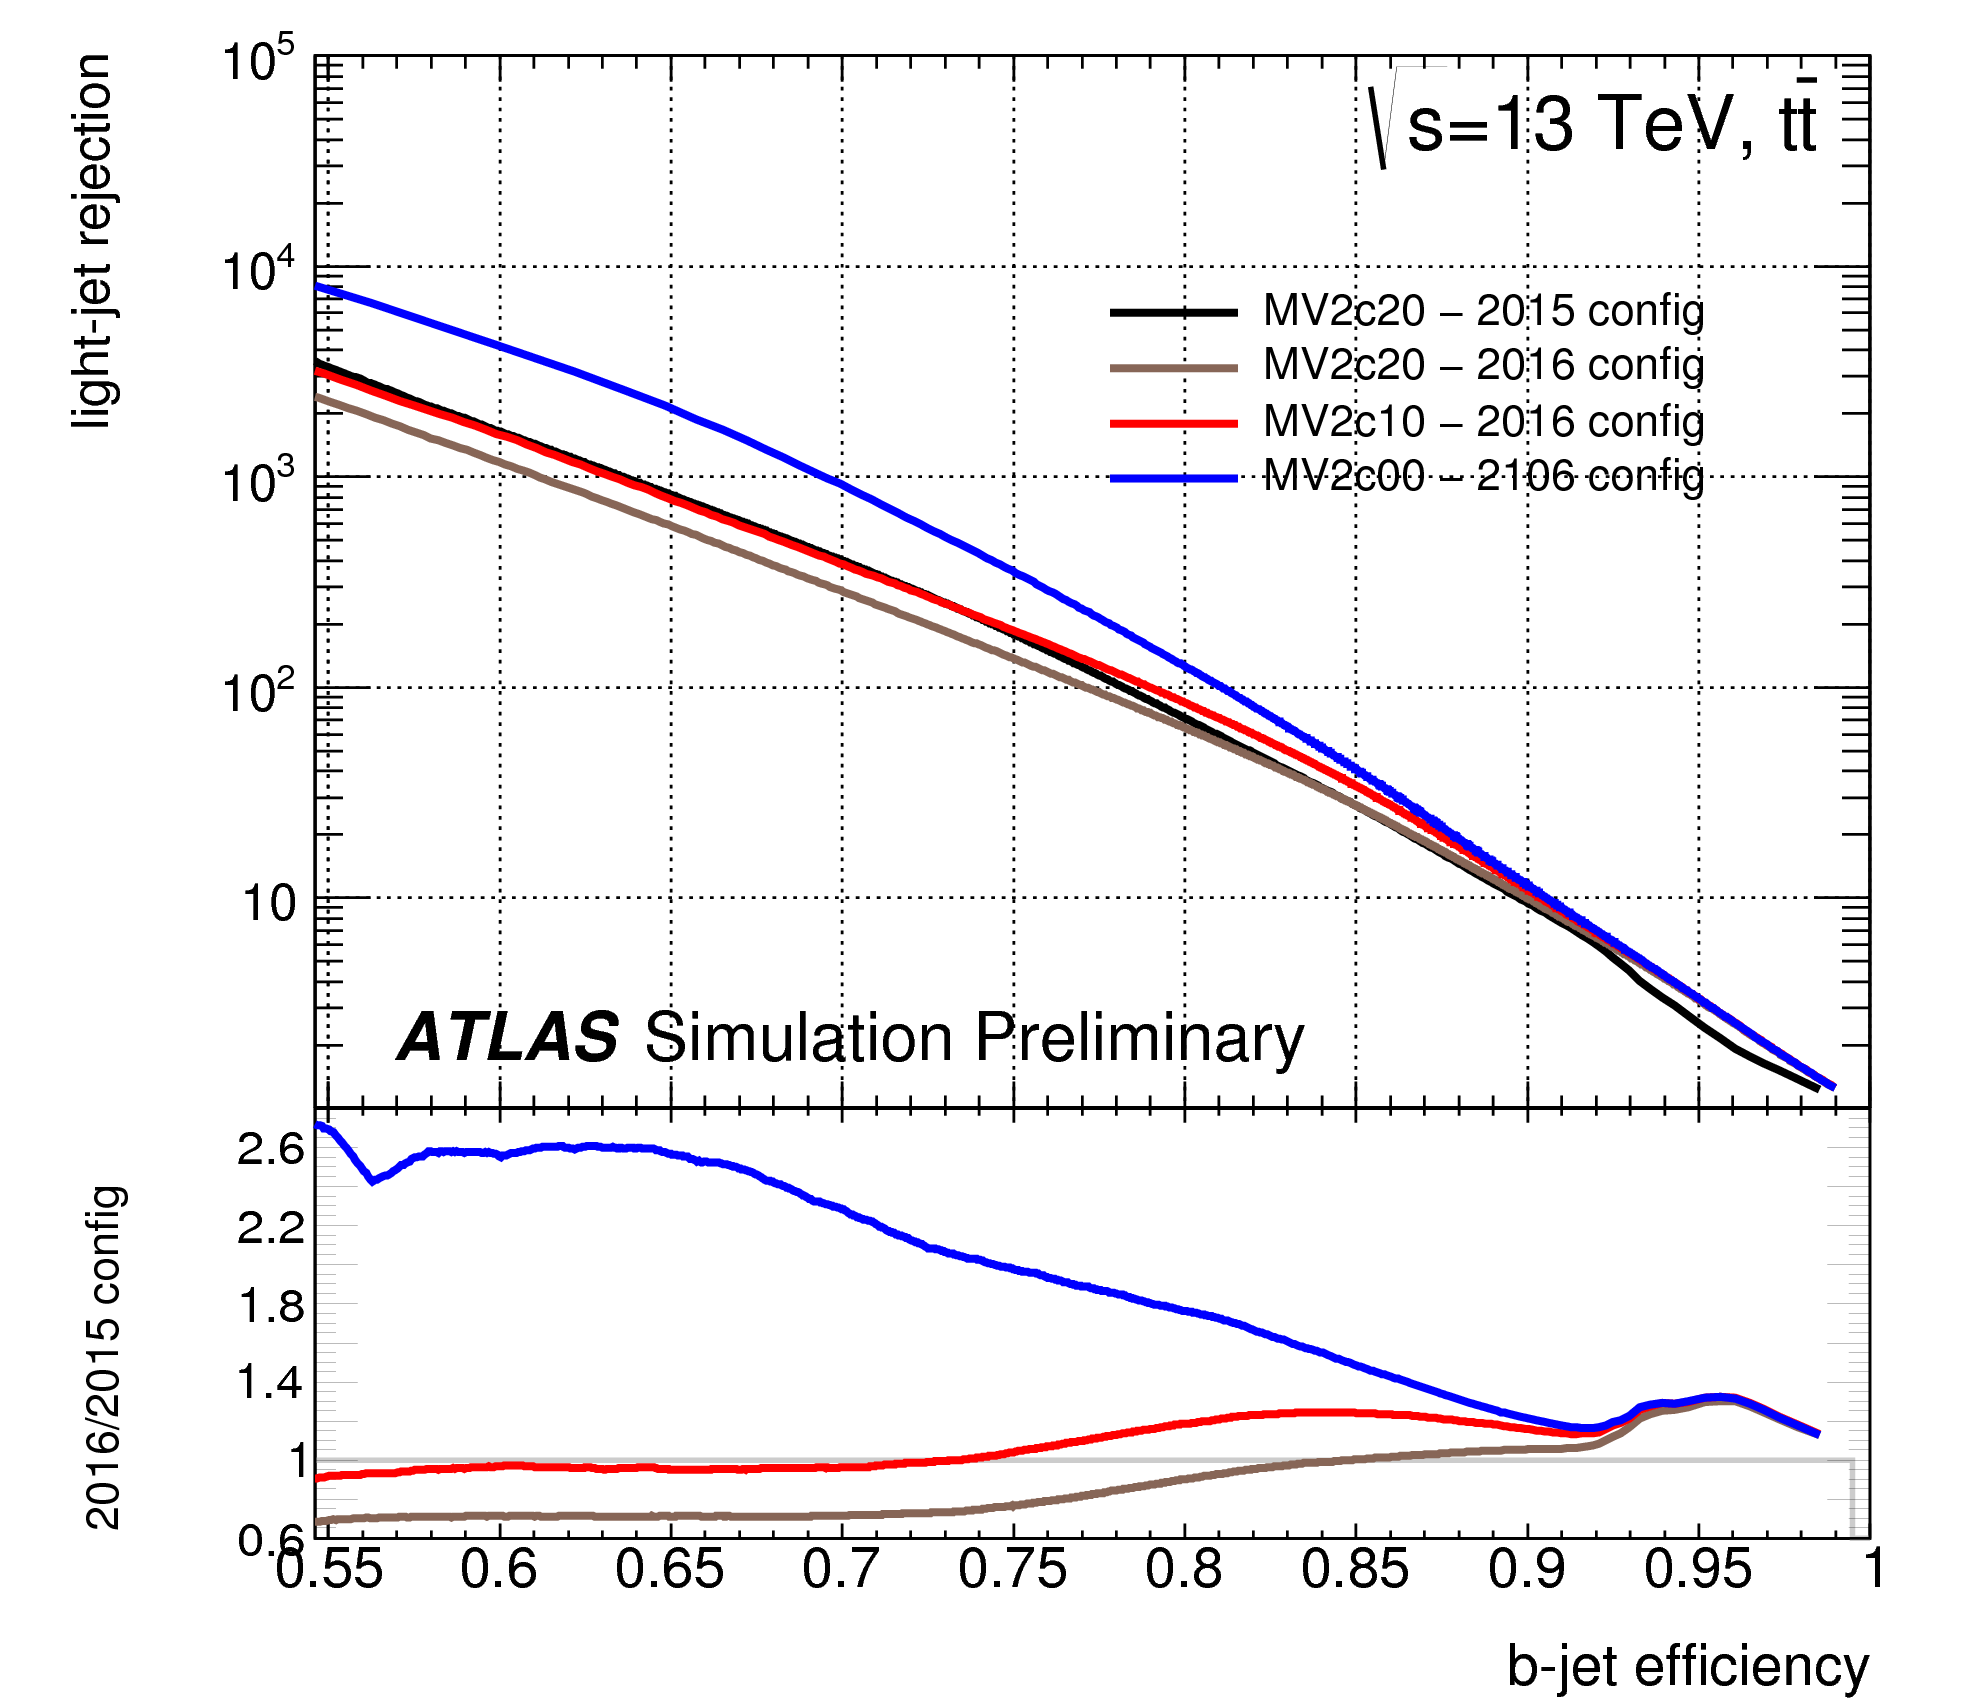
\includegraphics[width=0.45\textwidth]{MCobj/btag1}}\hspace{0.05\textwidth}
					\subfloat
						[\cj\ rejection versus \bj\ efficiency for $2015$ and $2016$ configurations of the MV2 b-tagging algorithm evaluated \ttbar\ events.]
						{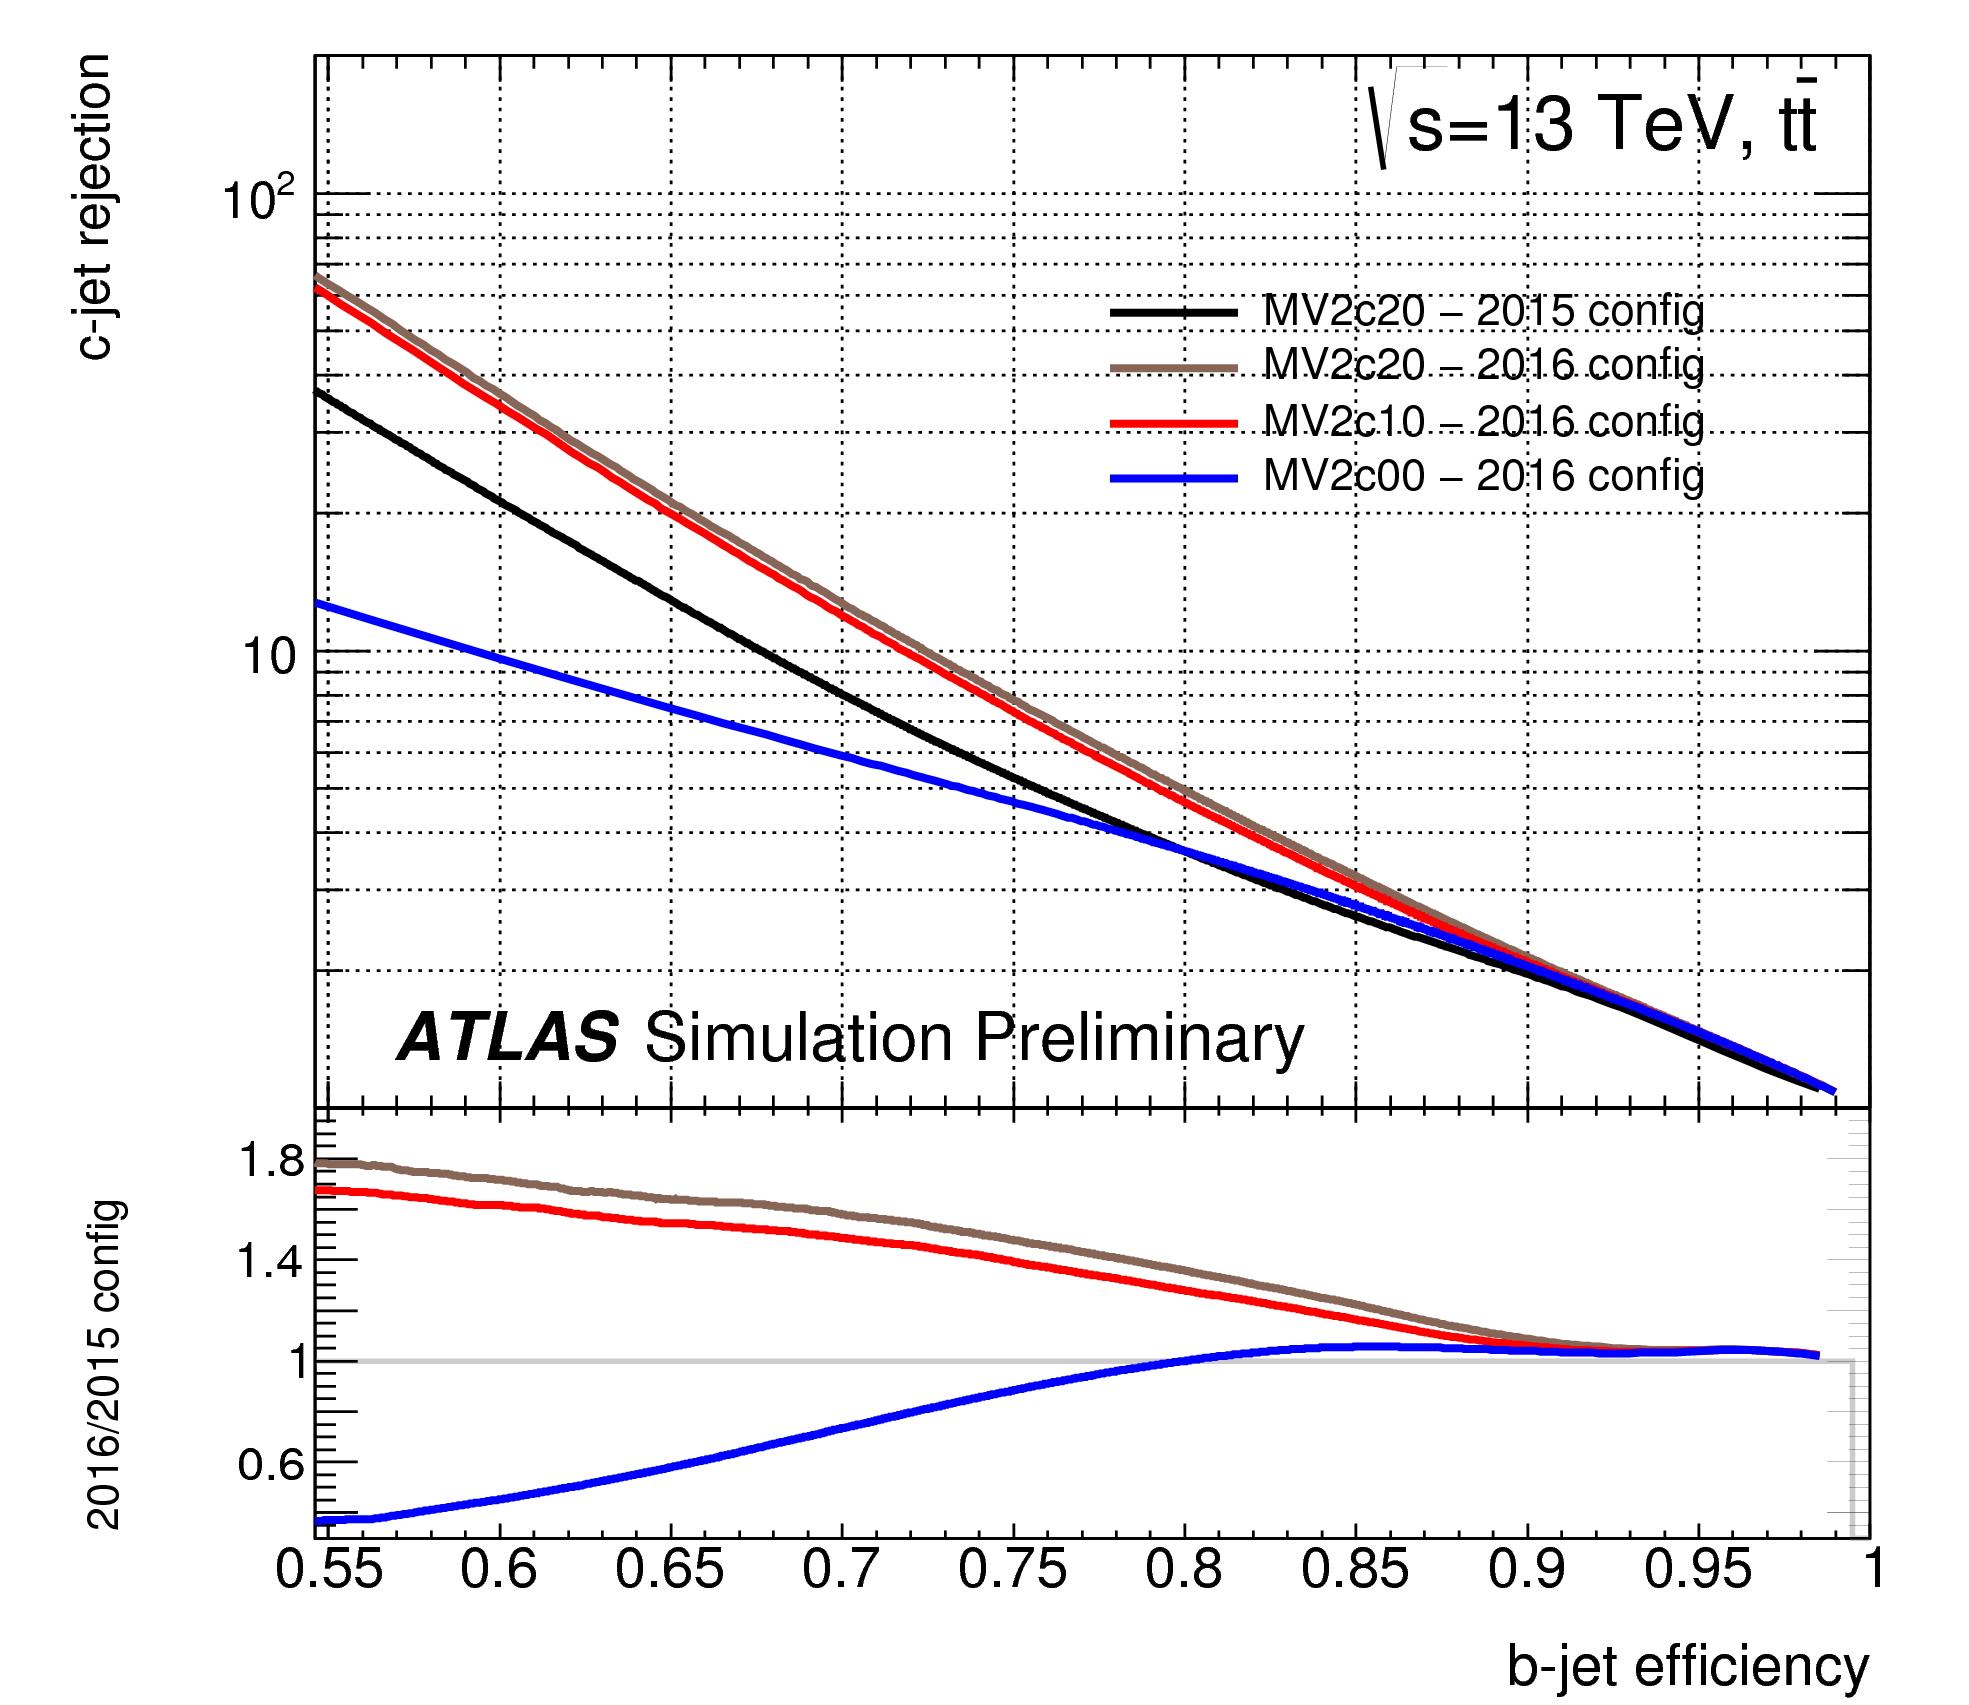
\includegraphics[width=0.45\textwidth]{MCobj/btag2}}
				\end{center}
				\caption{Performance of the MV2 tagger in \ttbar\ events. Various fractions of \cjs\ in the background training sample were considered (taken from~\cite{ATL-PHYS-PUB-2016-012}).}
				\label{fig:btagEff}
			\end{figure}

			Figure~\ref{fig:btagEff} shows the performances of different configuration of such tagger. In particular, the $b$-tagging efficiency is compared to the \cjs\ and light-jet rejection which can be defined as the inverse of the mis-tag rates. Furthermore, the more \cj\ there are in the background training sample the better the rejection will be, as opposite to the case where no \cjs\ are included. 



		\subsection*{Missing Transverse Energy, \met}

			\begin{figure}[!htb]
				\centering
				\includegraphics[width=.75\textwidth]{MCobj/METevdisp}
				\caption{\label{fig:METevdisp}ATLAS Event display for an event that has jets (blue solid lines) and \met (red dashed line) (taken from~\cite{METevdisp}).}
			\end{figure}

			As previously mentioned, particles like neutrinos or potential \ac{DM} candidates escape the \ac{ATLAS} detector. When these particles are produced a momentum imbalance in the transverse plane will characterise the event, as shown in Figure~\ref{fig:METevdisp}. Such quantity can be estimated using the four-momenta of all the visible detected objects in the event, and it is called missing transverse momentum, \ptmiss~\cite{ATLASMet2015}. The \ptmiss\ provides an estimate of the total momentum of the particles that escaped the \ac{ATLAS} detector and it is defined as it follows: 

			\begin{equation}
				\ptmiss = - \sum_i \vecpt^{i, \mathrm{obj}}
				\label{eq:ptmiss}
			\end{equation}

			\noindent Here, $\vecpt^{i, \mathrm{obj_i}}$ represents the transverse momentum of the $i$-th visible object in the event. The Missing Transverse Energy \met, is therefore defined as the magnitude of \ptmiss. 

			The \met\ is reconstructed by selecting calibrated hard objects to measure the missing transverse momentum in the event. In particular the $(x-y)$ components of the \met\ are calculated as it follows: 

			\begin{equation}
				E_{x(y)}^{\mathrm{miss}} = E_{x(y)}^{\mathrm{miss}, e} + E_{x(y)}^{\mathrm{miss}, \mu} + E_{x(y)}^{\mathrm{miss}, \tau} + E_{x(y)}^{\mathrm{miss, jets}} + E_{x(y)}^{\mathrm{miss}, \gamma} + E_{x(y)}^{\mathrm{miss,\,soft}}
				\label{eq:met_xy}
			\end{equation}

			where each object term is given by the negative vectorial sum of the momenta of the respective calibrated objects. In the analyses presented in this work, terms containing $\tau$ leptons were not considered as $\tau$ reconstruction was never explicitly performed. The \emph{soft term} is reconstructed from detector signal objects not associated with any object passing the selection cuts, \eg\ \ac{ID} tracks (track-based soft term) or calorimeter signals (calorimeter-based soft term). From the components in Equation~\ref{eq:met_xy} the magnitude of \met\ and the azimuthal angle $\phi^{\mathrm{miss}}$ are calculated as it follows:

			\begin{eqnarray}
				\met = \sqrt{ \left(E_{x}^{\mathrm{miss}}\right)^2 + \left(E_{y}^{\mathrm{miss}} \right)^2 } \qquad ; \qquad
				\phi^{\mathrm{miss}} = \arctan \left ( \frac{E_y^{\mathrm{miss}}}{E_x^{\mathrm{miss}}} \right )
			\end{eqnarray}

			The \met performance is studied in two complementary topologies, with and without genuine \met, such as $\Wboson \to e\nu$ and $\Zmm$, in both data and \ac{MC} in order to test the reconstruction algorithms and correct for any potential biases. 